\documentclass{article}
\usepackage{amsfonts}
\usepackage{multicol}
\usepackage[utf8x]{inputenc}
\usepackage{graphicx}
\usepackage{geometry}
\geometry{a4paper, total={170mm, 237mm}, left=20mm, top=20mm}
 
\title{ {\Large \textbf{DÉMONSTRATION AUTOMATIQUE EN COQ}} }
\date{}
\author{Quentin Garchery}

\setlength{\parindent}{0cm}


\begin{document}

\maketitle
\thispagestyle{empty}

\begin{center}
\normalsize sous la direction de \\

\vspace{7mm}

\begin{multicols}{2}
\large{Chantal Keller} \\
Maître de Conférences\\
Université Paris-Sud \\

\large{Valentin Blot} \\
Post-doctorant\\
Université Paris-Sud
\end{multicols}

\vspace{15mm}

\Large{Stage au Laboratoire de Recherche en Informatique\\
Université Paris-Sud / CNRS}


\vfill

\normalsize 20 août 2018

\end{center}
\newpage



\section{Introduction}

\subsection{Méthodes formelles}

Les méthodes formelles rassemblent différents outils informatiques qui permettent de formuler des propriétés mathématiques puis de les vérifier. La validité du résultat vérifié ne dépend alors que de ce logiciel de vérification. C'est dans ce cadre que G. Gonthier et B. Werner ont prouvé, en Coq, le théorème des quatre couleurs.\\

Les méthodes formelles s'étendent à la preuve de programme: il s'agit alors de vérifier qu'un programme correspond à sa spécification et permet donc d'aug-menter sa robustesse et sa fiabilité.
L'importance de la correction des logiciels est mise en avant dans le cas des systèmes critiques : le premier lancement d'Ariane 5 (1996) s'est soldé par un échec dû à un bug logiciel. Le compilateur Compcert est un exemple de programme certifié, sa vérification a été effectuée en Coq.\\

Parmi ces outils de vérification, on s'intéressera aux assistants de preuves et aux prouveurs automatiques. 

\subsection{Assistants de preuve}

Les assistants de preuves tels que Coq sont des outils puissants qui permettent d'exprimer des théorèmes complexes puis de les vérifier de manière interactive. Ils proposent à un utilisateur de formuler son problème puis de le démontrer, le rôle principal de l'assistant de preuve étant alors de vérifier que la preuve fournie est correcte.  La confiance accordée à ces outils dépend de la compréhension que l'on peut avoir dans son noyau, étant donné que c'est la partie sur laquelle repose la vérification. Cette compréhension est facilitée lorsque l'implantation de la logique de ce noyau est de taille réduite. \\

Pour une propriété donnée, l'utilisateur doit donc fournir une preuve parfaitement rigoureuse et exhaustive de la propriété ce qui peut rendre le processus de vérification long et fastidieux.



\subsection{Prouveurs automatiques}

Les prouveurs automatiques, quant à eux, ne demandent pas de preuves de la part de l'utilisateur. L'effort de certification est alors réduit à la formalisation du problème et dans certains cas le prouveur donne une trace de son exécution appelée certificat. \\

En contrepartie, la logique d'un prouveur automatique est plus limitée et/ou la réponse en temps fini n'est pas garantie.

\subsection{Motivations}

Nous aimerions bénéficier de l'automatisation des prouveurs automatiques dans un système expressif et sûr comme les assistants de preuves. Cette étape est faite par SMTCoq initialement. \\

Nous aimerions aussi que le développement à l'aide de cette automatisation soit adapté aux assistants de preuves: les preuves sont modulaires et peuvent reposer sur des lemmes précédemment démontrés. Pendant mon stage, je me suis attaché à améliorer ce point.


\subsection{Contexte}

L'assistant de preuve que nous utiliserons est Coq, sa logique du noyau se fonde sur le Calcul Inductif des Constructions. \\

SMTCoq est un plugin pour Coq qui utilise différents prouveurs automatiques. C'est un outil modulaire dans le sens où il est possible de rajouter d'autres prouveurs automatiques, ceux-ci n'ayant pas nécessairement le même format d'entrée ni le même format de sortie. SMTCoq permet d'une part d'améliorer l'automatisation de Coq. En effet, les preuves générées automatiquement par les prouveurs sont ensuite utilisée pour des preuves dans Coq. D'autre part, cela permet de vérifier les certificats fournis par les prouveurs automatiques et donc d'augmenter la confiance que l'on a dans ces outils.



\section{Preuves calculatoires en Coq}

\subsection{Règles de réduction en Coq}

La preuve par réflection utilise l'égalité interne à Coq: les termes sont considérés à réduction près. 
Aussi, à chaque nouvelle instance de Definition ou Fixpoint, une nouvelle règle de réduction est définie, ce qui est illustré dans l'exemple suivant par le fait que la preuve soit réduite au constructeur de l'égalité.\\

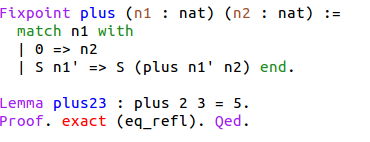
\includegraphics[height = 2.8cm]{refl.png}

Ce fonctionnement peut être exploité pour construire des preuves qui reposent sur un calcul effectué en Coq. 


\subsection{Un exemple: les formules conjonctives}
Donnons un exemple inspiré de \cite{coq_intro}.


Intéressons-nous au problème de mettre des formules booléennes avec seulement des conjonctions en forme de peigne. Avec $b_1, b_2, b_3, b_4$ des termes de type $bool$ et $\&$ la conjonction booléenne, on veut, par exemple, pouvoir passer de : 
\begin{center}
$ t = (b_1 \,\&\, b_2) \,\&\, (b_3 \,\&\, b4)$ \hspace{1cm} à   \hspace{1cm}  $t' = b_1 \,\&\, (b_2 \,\&\, (b_3 \,\&\, b4)). $
\end{center}

\subsubsection{Réification}

Pour cela, on a besoin de récupérer la structure du booléen $t$, c'est l'étape de réification. Ici, il s'agit de faire correspondre $t$ avec un terme du type inductif suivant :\\

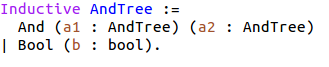
\includegraphics[height = 1.3cm]{andtree.png}

On définit alors récursivement la fonction d'évaluation $eval$ de ce type vers le type $bool$. \\

Il n'est pas possible d'écrire en Coq une fonction qui détermine la forme conjonctive d'un argument booléen. En effet, le type $bool$ n'ayant que deux constructeurs ($true$ et $false$), inspecter par pattern matching nous donnera un de ces deux constructeurs.\\

Une méthode est d'étudier la structure du terme en question à partir de sa représentation Ocaml sous-jacente. C'est l'approche utilisée par SMTCoq. \\

Il est aussi possible d'utiliser des tactiques qui renvoient un terme : \\

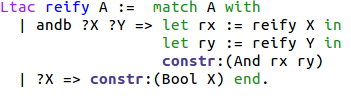
\includegraphics[height = 2cm]{reify.png}


Le terme $t$ réifié donne And (And (Bool b1) (Bool b2)) (And (Bool b3) (Bool b4)) et son évaluation est égale à $t$.

\subsubsection{Calcul et utilisation}

Sur le type $AndTree$, il est possible de définir une fonction $peigne$ qui renvoie l'arbre en argument mis sous forme de peigne. Le théorème de correction de cette fonction établit que 
\[ \forall a \in AndTree, \, eval (peigne (a)) = eval (a) \]

En combinant ces résultats, on peut définir une tactique $peignify$ qui met les formules conjonctives en forme de peigne. Cette tactique permet par exemple de démontrer le lemme suivant : \\

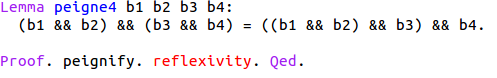
\includegraphics[height = 1.6cm]{peignify.png}

Cette preuve utilise le calcul de la fonction $peigne$ sur la réification du terme $t$ de type $bool$.







\newpage
\section{Fonctionnement d'un prouveur automatique}

Utilisation comme boite noire, un des intérêts de l'approche sceptique.\\


SMT-LIB, une interface commune aux prouveurs automatiques\\

SAT: \\
cnf : conjonction de clauses \\ 
clause : disjonction de littéraux \\
littéral : atome ou négation d'atome \\
atome : ensemble (fini?) fixé \\

SMT: \\
on peut voir les lemmes de la théorie comme des atomes. Ils sont utilisés par les prouveurs. \\
Fonctionnement d'un smt prouveur :\\
-faire sat sur la formule en considérant les atomes comme indéfinis \\
-en déduire une intanciation qui marche, sinon renvoyer unsat \\
-envoyer cette intanciation aux prouveurs \\
-si tous les prouveurs renvoient vrai alors c'est sat \\
-sinon les prouveurs donnent un lemme additionnel \\
-rajouter ce lemme et recommencer (il y a un nombre fini d'instanciation des atomes)\\ 



Les certificats de zChaff:\\
-maintiennent un état des variables \\
-donnent un ordre d'exécution (L : 2) \\
-définissent des clauses apprises au début du fichier par résolution \\
-définissent des commandes fixant la valeur d'une variable (Var : 5) à vrai (V : 1) ou faux (V : 0) \\
-définissent une clause de conflit (qui explicite les littéraux de conflit)\\

Il y a différentes stratégies pour l'implantation de dpll, on peut choisir de donner une priorité plus importante à la théorie ou aux solveur SAT, à plusieurs niveaux, priorité des règles de Basic dpll. 

La résolution de deux clauses utilise une dérivée de la fonction merge de merge sort.

\newpage 
\section{Présentation de SMTCoq}

\subsection{SMTCoq, une interface sceptique entre Coq et les prouveurs automatiques}

Pour améliorer l'automatisation de Coq et y intégrer l'utilisation de prouveurs automatiques, il y a principalement deux approches.

\begin{multicols}{2}
\begin{center}
Approche autarcique\\
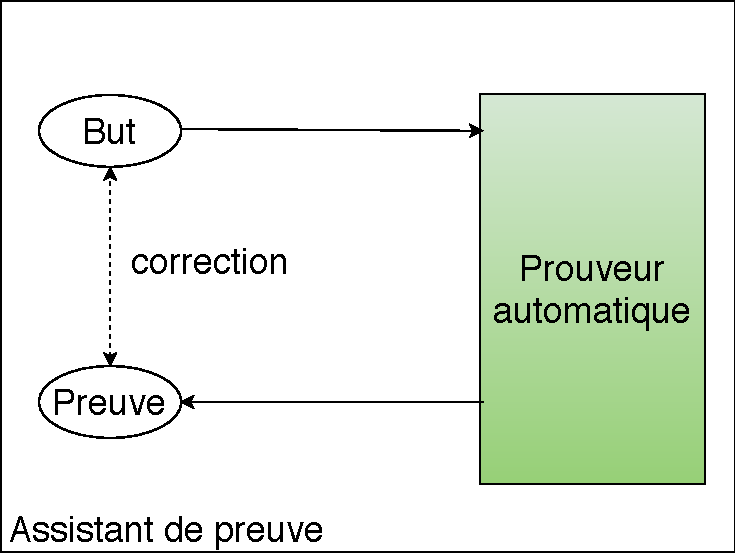
\includegraphics[height=5cm]{1_Autarcique.pdf}\\
Approche sceptique\\
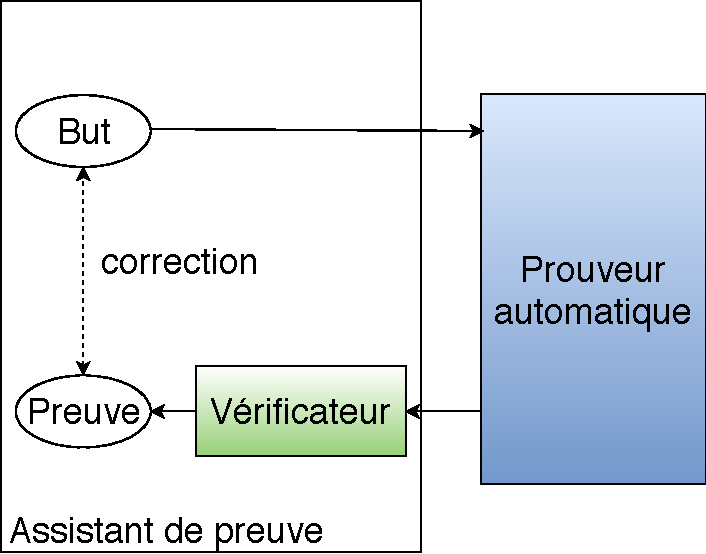
\includegraphics[height=5cm]{2_Sceptique.pdf}\\

\end{center}
\end{multicols}

L'approche autarcique consiste à vérifier le code du prouveur automatique à l'intérieur de l'assistant de preuve. L'avantage de cette méthode est qu'une fois cette vérification faite, on sait que chaque appel du prouveur automatique nous renverra une preuve correcte. \\

Dans l'approche sceptique, le certificat renvoyé par le prouveur automatique est vérifié à chaque appel de celui-ci. Cela permet d'une part de ne pas figer l'implantation du prouveur automatique puisque ce n'est pas son code qui est vérifié mais sa sortie. D'autre part, l'effort de certification est plus restreint : pour un certificat fixé, il faut vérifier que celui-ci correspond bien à une preuve du but.\\

SMTCoq a une approche sceptique de la vérification des prouveurs automatiques.

\subsection{Fonctionnement de SMTCoq}

\subsubsection{Amélioration de la confiance}


SMTCoq propose une commande Coq de reconstruction d'une preuve effectuée par un prouveur automatique.

\begin{center}
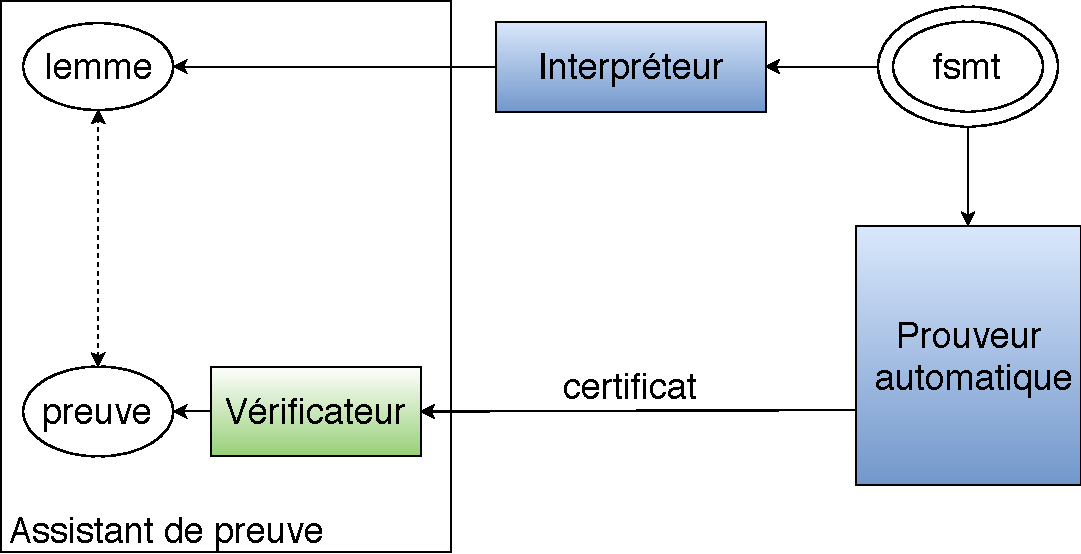
\includegraphics[height=5cm]{Confiance.pdf}
\end{center}

 Cette commande prend en paramètre un fichier 'fsmt' décrivant le lemme (typiquement écrit en SMT-LIB) et le certificat fourni par un prouveur automatique. Le lemme Coq est reconstruit à l'aide de l'interpréteur de SMTCoq et la preuve est reconstruite grâce au vérificateur. Une fois la reconstruction faite, la vérification que la preuve correspond bien au lemme est laissée à Coq. \\

Puisqu'un nouveau lemme Coq est créé, l'utilisateur peut vérifier que c'est bien le but qu'il voulait prouver. Ainsi, la confiance dans les prouveurs automatiques est améliorée: on peut vérifier la réponse du prouveur.


\subsubsection{Amélioration de l'automatisation}

SMTCoq définit également des tactiques Coq, une par prouveur automatique : "zchaff" et "verit". \\


\begin{center}
    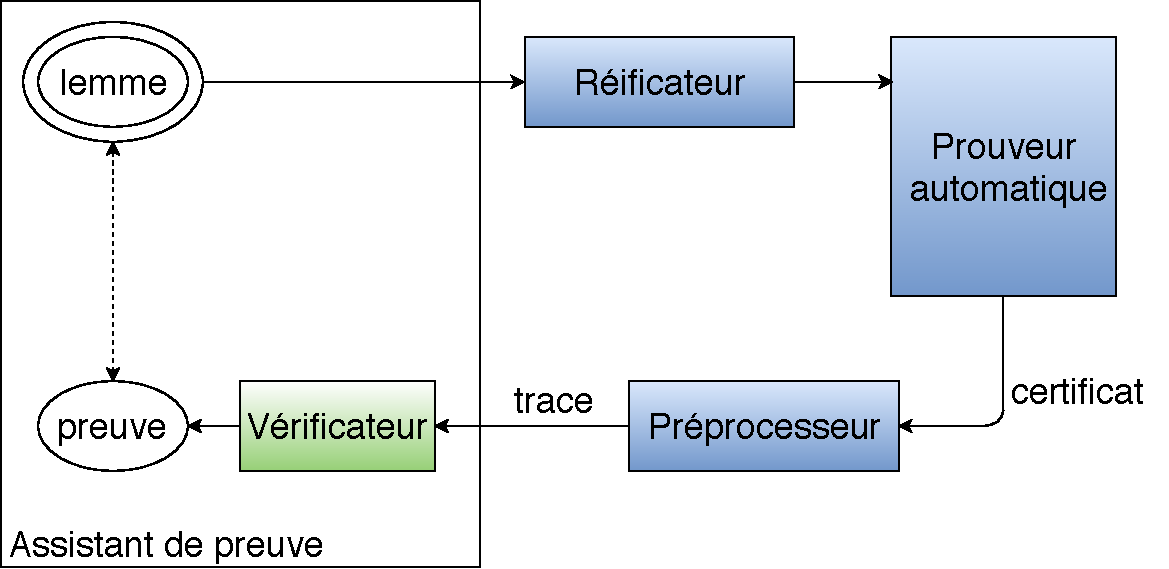
\includegraphics[height=5cm]{Automatisation.pdf}
\end{center}

La première étape est la réification, le lemme est traduit dans l'AST des formules acceptées par SMTCoq. Le prouveur automatique est appelé à partir de cet AST. En cas de succès de ce prouveur, on obtient un certificat de preuve. 
Il s'agit ensuite de rejouer ce certificat en Coq, on utilise le vérificateur de SMTCoq. Il faut pour mettre le certificat dans une forme adaptée qu'on appelle trace. Cette phase de préprocessing consiste en une étape de parsing du certificat qui se souvient des sous-formules déjà rencontrées (hash-consing) à l'aide de tables de hashage.  Il y a aussi une étape d'adaptation de ces certificats. En effet, les prouveurs automatiques peuvent parfois ne pas mentionner une étape de la preuve qu'il faut alors construire. De plus, il faut pouvoir adapter les certificats à fournis par le prouveur automatiques qui peuvent reposer sur une logique différente de celle de Coq. \\

Ces tactiques permettent à l'utilisateur Coq de profiter de l'automatisation de différents prouveurs.

\subsubsection{Cas d'application de SMTCoq}

Dans les deux cas, les formules acceptées sont les formules logiques propositionnelles en forme prénexe. À cela se rajoutent toutes les combinaisons des théories suivantes : arithmétique linéaire sur $\mathbb{Z}$, égalité et fonctions non-interprétées, vecteurs de bits et théories des tableaux. 

\subsection{Exemples d'utilisation de SMTCoq}

\subsubsection{Exemple de la commande de reconstruction}

SCHÉMA Verit\_Theorem puis Print du théorème créé.

\subsubsection{Exemple de la tactique verit}

SCHÉMA utilisation de verit seulement (pas de print du résultat)


\newpage
\section{Certificats et vérificateur}

\subsection{Certificat de verit}

Les certificats de veriT:\\
int:(type (clause) dep) \\

SCHÉMA VERIT\_CERTIF

explication du certificat, clause vide

\subsection{La fonction $checker$}

Le vérificateur définit une fonction Coq $checker$ qui est définie récursivement sur son paramètre trace qui est un tableau de $step$ et qui maintient un tableau de clauses appelées état. Initialement l'état contient des valeurs triviales et à chaque appel de checker, une nouvelle $step$ est consommée, $checker$ met alors à jour l'état courant.

Une $step$ est représentée par un type somme, chaque constructeur regroupant plusieurs étapes qui peuvent apparaître dans le certificat.

SCHÉMA STEP : inductive step = ImmBuildProj c par $|$ EqTr f1 ... fn f

Le constructeur ImmBuildProj par exemple regroupe les règles not\_implies1 et not\_implies2. EqTr est la transitivité de l'égalité : f1 .. fn et f doivent suivre le chéma de la transitivité : par exemple f1 = ~(a1=a2) f2= ~(a2=a3) ... fn=~(an=a{n+1}) et f = (a1 = a{n+1}).

Pour chaque constructeur $X$ de $Step$ correspond une fonction $schecker$ qui est appelée par $checker$ lorsque le constructeur $X$ est rencontré. $schecker X$ donne une nouvelle clause valide à partir de celles déjà présentes dans l'état (et des tables de hashage, etc). Par exemple le $schecker$ de EqTr f1 ... fn f avec f1 ...fn et f comme ci-dessus donne la tautologie (f1 \/ ... \/ fn \/ f). $checker$ utilise aussi des positions qui indiquent où enregistrer cette nouvelle clause dans le tableau état. \\

Enfin $checker$ utilise un paramètre de position. Lorsque tous les calculs de mise à jour de clause sont faits, checker regarde à la position indiquée par l'état et renvoie vrai si la clause est vide à cet endroit et faux sinon.

\subsection{Exemples de certificats et de vérificateurs}
\subsubsection{resolution chains}
C'est simplement une liste de clause.
Le schecker associé fait un fold dessus en appliquant la règle de resolution dessus. Cette règle est refutationnellement complète.

\subsubsection{nor\_certif}
Il implémente la règle $\neg (A_1 \vee A_2 \vee ... \vee A_n) \Rightarrow ~A_i$

\subsubsection{congruence theory}
Qui implémente les règles de transitivité et de congruence.

\subsection{Théorème de correction}

Le vérificateur repose sur le théorème de correction suivant :

\[ \forall l \, \forall t. \quad checker \, t = true \quad \Rightarrow \quad interp \, l \]








\section{Adaptation des certificats}

Afin de ne pas avoir à rajouter des binders dans les proof witness de veriT, nous avons choisi de faire un
preprocessing dans les certificats renvoyés par veriT.
Les règles instance apparaissent sous la forme suivante :
     (forall\_inst (or (not lemma) lemma\_inst) id)
où lemma est un des lemmes rajoutés par l'utilisateur et lemma\_inst est une instance de ce même lemme.

Pour chacune de ces règles instances, on garde une trace du lemme auquel elle se réfère puis on modifie la valeur
de cette règle: ce n'est plus (or (not lemma) lemma\_inst) mais seulement (lemma\_inst). En contrepartie, les règles
de résolution qui utilisent à la fois une de ces règles instances et le lemme associé sont réduites à seulement
l'instance du lemme.

Exemple :
si on a ensuite
(resolution (thm) id1 id2 id3)
et que id2 donne la règle instance écrite ci-dessus et que id3 donne la règle
(input (lemma))
alors on remplace cette règle résolution par une règle de résolution ayant id1 et id2.

On a fait également attention au fait que les règles temporaires de veriT donnent des alias des lemmes de départ
et qu'après une règle forall\_inst il y a une règle qui transforme le OR interne en OR externe.

\renewcommand\refname{Bibliographie}
\nocite{*}
\bibliography{biblio}{}
\bibliographystyle{plain}

\end{document}
